\documentclass[aps,prl,twocolumn,showpacs,amsmath,amssymb]{revtex4-1}
%\documentclass[aps,prl,twocolumn,showpacs,preprintnumbers,amsmath,amssymb,citeautoscript]{revtex4-1}
%\documentclass[prl,showpacs,amssymb,amsmath,twocolumn]{revtex4-1}
%%%%%%%%%%%%
\usepackage{bookmath} % definitions and shortcuts
%%%%%%%%%%%%
\usepackage{graphicx}
\usepackage{amsmath}
\usepackage{color}
\newcommand{\blue}{\textcolor{blue}}
\newcommand{\red}{\textcolor{red}}
\newcommand{\cecoin}{CeCoIn$_5$} 
\def\opp#1{{\overline{ #1}}}


\bibliographystyle{apsrev4-1}
%~~~~~~~~~~~~~~~~~~~~~~~~~~~~~~~~~~~~~~~~~~~~~~~~~~~~~~~~~~~~~~~~~~~~~~~~~~~~~~~%
\begin{document}
%~~~~~~~~~~~~~~~~~~~~~~~~~~~~~~~~~~~~~~~~~~~~~~~~~~~~~~~~~~~~~~~~~~~~~~~~~~~~~~~%
\title{Electronic Spin Susceptibility Enhancement in Pauli Limited Unconventional Superconductors}

\author{Ben Rosemeyer}
\author{Anton~B.~Vorontsov}

\affiliation{Department of Physics, Montana State University, Montana 59717, USA}

\date{\today}

\begin{abstract}
%
We calculate the wave-vector dependent electronic spin susceptibility 
$\chi_{\alpha\beta}(\vq, \vH_0)$ 
of a superconducting state in uniform magnetic field $\vH_0$. 
We consider Pauli limited materials with $d$-wave symmetry, and a 2D cylindrical 
electronic Fermi surface.  
We find that both longitudinal and transverse components of the susceptibility tensor are enhanced over their
normal state values.  
We identify several wave vectors, connecting field-produced hot spots on the Fermi surface, 
that correspond to the maximal enhancement of either $\chi_\perp$ or $\chi_\parallel$ components. 
The enhancement of susceptibility is a result of the unconventional order parameter and is the 
largest 
in the high-field low-temperature region of the $T$-$H$
phase diagram. 
These results can help explain the observed anomalous high-field phase in heavy-fermion \cecoin. 
%
\end{abstract} 

\pacs{74.20.Rp,74.25.Dw, \dots} % \red{MORE?,DIFFERENT?} }

%74.20.Rp 	Pairing symmetries (other than s-wave) 
%74.25.Dw 	Superconductivity phase diagrams 


\maketitle


%~~~~~~~~~~~~~~~~~~~~~~~~~~~~~~~~~~~~~
%\emph{Introduction.}
%~~~~~~~~~~~~~~~~~~~~~~~~~~~~~~~~~~~~~
%
The interplay of different orders, simultaneously present in the same system, 
is of a great interest to physics community and beyond. 
Such interactions present another level of complexity in emergent systems. 
They offer insight into the properties of the ordered phases, but also 
often pose a great challenge both mathematically 
and conceptionally.\cite{x}
The two most widely studied orders, that often appear together in many systems, 
are superconductivity and magnetism, both having their origin tightly 
connected to the behavior of the quantum mechanical spin. 
The behavior of these orders have been investigated under many different conditions. 
Ferromagnetic order and singlet superconductivity avoid each other since they have opposite spin 
structures\cite{x}; 
on the contrary triplet superconductivity is much less sensitive to the ferromagnetism\cite{x}; 
antiferromagnetic order with spatial period much smaller than the superconducting coherence length 
does not interfere with superconductivity, and the two orders may easily appear together\cite{x},  
and in some cases unconventional superconducting and spin-density wave orders even attract each other\cite{x}. 

Despite this great amount of knowledge, the 
interplay of antiferromagnetism (AFM) and superconductivity (SC) still often challenges
our understanding of this phenomenon, for various reasons. 
For example, materials such as cuprate oxides have unusual normal state properties \cite{x}, 
whereas iron-based superconductors have complex orbital multiband structure\cite{x}. 

%%%%%%%%%%%%%%%%%%%%%%%%%%%%%%%%%%%%%%%%%%%%%%%%%%%%%%%%%%%%%%%%%%%%%%%%%%%%%%%%%
\begin{figure}[t]
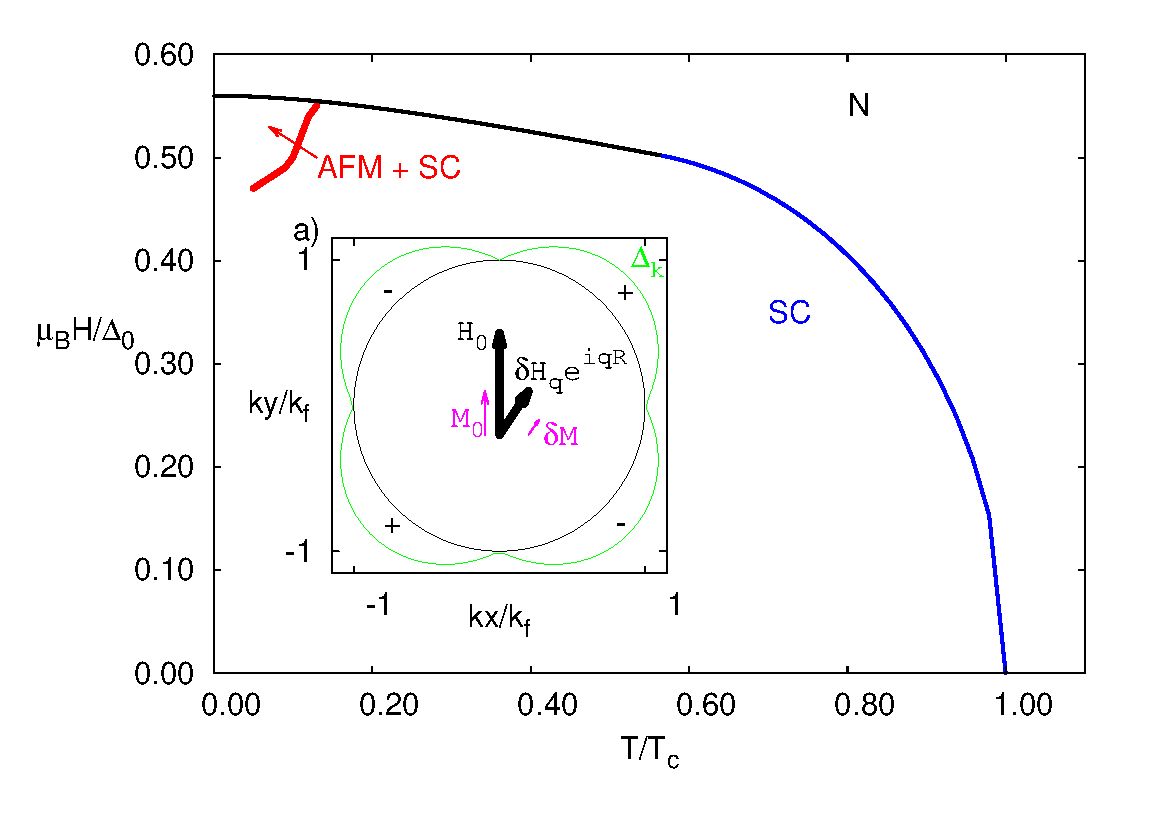
\includegraphics[width = 0.5\linewidth]{Fig1.eps}
\caption{ \label{fig:model}
(Color online) 
We consider 2D electrons with circular Fermi surface (FS). 
The $d$-wave order parameter $\Delta_\vk \propto \sin 2\theta_\vk $ is also shown. 
Magnetic field has large uniform component $\vH_0$ and spatially varying perturbation $\delta \vH_\vq$
with wave vector $\vq$. 
}
\end{figure}
%%%%%%%%%%%%%%%%%%%%%%%%%%%%%%%%%%%%%%%%%%%%%%%%%%%%%%%%%%%%%%%%%%%%%%%%%%%%%%%%%

In this paper we investigate microscopic origin of the 
attraction between magnetism and unconventional superconductivity 
in $d$-wave materials. 

One other, interesting and relatively recent example, is heavy-fermion material 
\cecoin, which manifests a coexistent AFM and superconducting state (Q-phase) \cite{cecoin5_Bianchi, cecoin5_Kenzelmann, cecoin5_Kenzelmann2}
in the high-field low-temperature limit. 
Experimental results for \cecoin\ indicate that this co-existence is the result of 
strong attraction between superconducting unconventional $d$-wave order, 
and the AFM state\cite{cecoin5_Bianchi,cecoin5_Kenzelmann,cecoin5_Kenzelmann2}. 
The Q-phase and magnetism disappear when superconductivity is suppressed at the upper critical field $H_{c2}$ 
through a first order transition to the normal state. 
The magnetic order appears inside the SC state through a second order transition. 
Moreover, although the normal state of \cecoin\ is non-magnetic, the proximity to magnetic 
instability can be demonstrated by applying doping to induce it, or pressure, to destroy it.\cite{doped_cecoin5, cecoin5_Kenzelmann, cecoin5_Kenzelmann2, cecoin5_magnetism_chapter} 

\red{To be edited more...} 

Other results for \cecoin\ show that the magnetic ordering wave vector in the
Q-phase displays little or no dependence on field (within experimental error),
which indicates a relatively small or non-existent interaction with the flux
lattice \cite{cecoin5_Kenzelmann2}. This phenomenon has not been directly
addressed in many of the current theories. Our findings indicate that this
behavior is more consistent with the longitudinal component of suscep	tibility
rather than the transverse. This is another area of study which has not been
very thouroghly analyzed.

Many theories have been proposed to explain the experimental results seen in
\cecoin, including various manifestations of the FFLO state where the
superconducting order parameter oscillates in real space.
\cite{sc_sdw_anton,mag_afm_fflo_sigrist,fflo_pen_depth,sc_afm_kato,sc_afm_ikeda,sdw_vortex}.
The FFLO state has long been believed to offer the possibility of magentic
order, however, the predicted field dependence of the ordering vector is not
seen in experiment, and recent experiments point to a homogeneous gap function
\cite{cecoin5_Kenzelmann2,cooperPairsCeCoIn5}.

Yet other theories offer insight but leave many questions unanswered. Such as:
How does the ordering wave vector change with applied field? What are the
necessary conditions on the order parameter? And what roles do the transverse
and longitudinal components of the magnatism play? Here we provide a first
principles approach to these problems by calculating the magnetic
susceptibility of itinerant electrons in the D-wave superconducting state. 
In this paper we investigate the microscopic underlay of such interaction. 





%~~~~~~~~~~~~~~~~~~~~~~~~~~~~~~~~~~~~~
%\emph{Model.}
%~~~~~~~~~~~~~~~~~~~~~~~~~~~~~~~~~~~~~
%
To investigate the interplay of superconductivity and magnetic order in external field,  
we consider mean-field SC Hamiltonian of 2D electrons with cylindrical FS, interacting with uniform magnetic field $\vH_0$
through Zeeman term: 
$
\cH = \cH_{0} + \cV  
$
\bea
\label{eq:modelH} 
\cH_{0} = \sum_{\vk \mu} \xi_\vk c^\dag_{\vk \mu} c_{\vk,\mu} 
+ \sum_\vk \left( \Delta_\vk c_{\vk,\uparrow}^\dag c_{-\vk,\downarrow}^\dag + h.c. \right) 
\\
+ \mu_\sm{B} \sum_{\vk \mu \nu} c^\dag_{\vk\mu} \, \vsigma_{\mu\nu} \vH_0 \, c_{\vk\nu}  
\nonumber  
\eea
and the interaction is due to a $\vq$-dependent perturbation of the magnetic field $\delta\vH(\vR) = \delta\vH_\vq e^{i\vq\cdot\vR}$, 
$\cV = \mu_\sm{B} \sum_{\vk \mu \nu} c^\dag_{\vk+\vq \mu}  \, \vsigma_{\mu\nu} \delta\vH_\vq \, c_{\vk \nu}  $.
The electronic dispersion in the normal state is $\xi_{\vk}=\frac{\vk^2}{2m^*}-\epsilon_F$, 
and $\mu_\sm{B}$ is the magnetic moment of electron.  
The resulting magnetization has uniform part and linear response to perturbation:
\bea
M_\alpha(\vR) = M_{0\alpha}(\vH_0) + \delta M_\alpha(\vR)
\\
\delta M_\alpha(\vR) = \chi_{\alpha\beta} (\vq) \delta H_\beta e^{i\vq \cdot \vR}
\eea
given by the standard expressions~\cite{mahan}: \red{Ben, check!!!}
\bea
&& \vM_0(\vr,t) = \mu_\sm{B} \langle \vS(\vr,t) \rangle_0 \,,
\\
&& \chi_{\alpha\beta}(\vr, t)= -\frac{i \mu_\sm{B}^2}{\hbar} 
\langle [ S_\alpha(\vr,t), S_\beta(0,0) ] \theta(t) \rangle_0 
\\
&& \chi_{\alpha\beta}(\vq)=  
\int d^3 r e^{-i\vq\vr} \int\limits_{0}^{+\infty} dt \, e^{-0^+ t} \,  
\chi(\vr, t)
\label{eq:susdef}
\eea
with 
$\vS(\vr,t) = \sum_{\mu \nu} \psi^\dag_\mu(\vr,t) \, \vsigma_{\mu\nu} \, \psi_{\nu}(\vr,t)$,  
$\psi_{\nu}(\vr,t) = \sum_\vk c_{\vk \nu} (t) \varphi_\nu(\vr)$, 
$c_{\vk \nu} (t) = e^{i\cH_0 t} c_{\vk \mu} e ^{-i \cH_0 t}$, 
and 
the subscript $0$ indicating the average over ensemble given by the Hamiltonian (\ref{eq:modelH}). 

The temperature and magnetic field dependence of the uniform magnetization $\vM_0$
is known, eg.\ref{ABV_Graf},
and here we are interested in the susceptibility $\chi_{\alpha\beta}(\vq)$, since 
it determines the magnetic instability into 
an SDW (spin-density wave) state, 
or responsible for RKKY-type interaction between localized moments. 
To calculate the susceptibility (\ref{eq:susdef}) in superconducting state, we diagonalize 
the Hamiltonian (\ref{eq:modelH}) by the 
Bogoliubov transformation, 
$c_{\vk \mu} = u_\vk \gamma_{\vk \mu} + (i\sigma_2)_{\mu\nu} v_\vk^* \gamma^\dag_{-\vk \nu} $
%
\be 
\cH_0 = \sum_{\vk \mu} \epsilon_{\vk \mu} \gamma^\dag_{\vk \mu} \gamma_{\vk \mu} \,,
\quad
\epsilon_{\vk\mu} =\sqrt{ \xi_{\vk}^2 + \Delta_{\vk}^2 }  \pm \mu_\sm{B} H_0 
\ee 
with coefficients of the transformation being in fact spin-independent, 
$\epsilon_\vk = \sqrt{ \xi_{\vk}^2 + \Delta_{\vk}^2 }$, 
\be
u_{\vk}= \sqrt{\frac{1}{2}\left( 1+\frac{\xi_{\vk}}{\epsilon_\vk}  \right)} \,, \quad 
v_{\vk}= \sgn(\Delta_\vk) \sqrt{\frac{1}{2}\left( 1-\frac{\xi_{\vk}}{\epsilon_\vk} \right)}
\ee
%u_{\vk}=\sqrt{\frac{1}{2}\left( 1+\frac{\xi_{\vk}}{\sqrt{\Delta_{\vk}^2+\xi_{\vk}^2}} \right)} \\
%v_{\vk}= \sgn(\Delta_\vk) \sqrt{\frac{1}{2}\left( 1-\frac{\xi_{\vk}}{\sqrt{\Delta_{\vk}^2+\xi_{\vk}^2}} \right)}

In the presence of external magnetic field $\vH_0$ the spin-rotational symmetry is broken even in magnetically 
isotropic system. 
Now one has to distinguish between two possibilities for the direction of the wave-vector dependent magnetization: 
(a) $\delta \vM(\vq) \parallel \vH_0$ (longitudinal response), and 
(b) $\delta \vM(\vq) \perp \vH_0$ (transverse response). 
The general expressions for the two components of the susceptibility are: 
%%%%%%%
\begin{widetext}
\bea
\label{eq:chi}
\chi_{\parallel}( \vq ) = -\mu_\sm{B}^2 \sum\limits_{\vk\mu} 
\frac{ [ f(\epsilon_{\vk_-\mu}) -f(\epsilon_{\vk_+\mu}) ] ( u_{\vk_+}u_{\vk_-}+v_{\vk_+}v_{\vk_-} )^2} 
     { \epsilon_{\vk_-\mu}-\epsilon_{\vk_+\mu} } 
-\frac{ [ 1-f(\epsilon_{\vk_-\mu})-f(\epsilon_{\vk_+\opp{\mu}}) ] ( u_{\vk_+}v_{\vk_-}-v_{\vk_+}u_{\vk_-} )^2 }
	{ \epsilon_{\vk_-\mu}+\epsilon_{\vk_+\opp{\mu}} }
\\
\chi_{\perp}( \vq ) = -\mu_\sm{B}^2 \sum\limits_{\vk\mu} 
\frac{ [ f(\epsilon_{\vk_-\mu})-f(\epsilon_{\vk_+\opp{\mu}}) ] ( u_{\vk_+}u_{\vk_-}+v_{\vk_+}v_{\vk_-} )^2 }
	{ \epsilon_{\vk_-\mu}-\epsilon_{\vk_+\opp{\mu}} } 
-\frac{ [ 1-f(\epsilon_{\vk_- \mu})-f(\epsilon_{\vk_+\mu}) ] ( u_{\vk_+}v_{\vk_-}-v_{\vk_+}u_{\vk_-} )^2 }
	{\epsilon_{\vk_-\mu}+\epsilon_{\vk_+\mu}} \nonumber
\eea
\end{widetext}
%%%%%%%
where $\chi_0 = 2 \mu_\sm{B}^2 N_F$ is Pauli susceptibility in the normal state, 
$f(\epsilon) = [ \exp(\epsilon/T)+1 ]^{-1}$ is the Fermi distribution, 
and momenta are shifted by the magnetization wave vector $\vk_\pm = \vk \pm \vq/2$. 
Notation $\opp{\mu}=\mp1$ means spin state opposite to $\mu = \pm1$. 

%~~~~~~~~~~~~~~~~~~~~~~~~~~~~~~~~~~~~~
%\emph{Results.}
%~~~~~~~~~~~~~~~~~~~~~~~~~~~~~~~~~~~~~
%
In the normal state, by setting $\Delta_\vk = 0$ in the general expression above, one obtains the familiar 
Lindhard function,  
\bea
\label{eq:chiN}
\chi^N_{\parallel}(q) =- \mu_\sm{B}^2\sum\limits_{\vk\mu} 
	\frac{ f(\xi_{\vk\mu})-f(\xi_{\vk+\vq \mu})}
	{ \xi_{\vk \mu}-\xi_{\vk+\vq \mu} } 
	\\
\chi^N_{\perp}(q) =- \mu_\sm{B}^2 \sum\limits_{\vk \mu} 
	\frac{ f(\xi_{\vk\mu})-f(\xi_{\vk+\vq \opp{\mu}}) }
	{ \xi_{\vk \mu}-\xi_{ \vk+\vq \opp{\mu}} }  \nonumber
\eea
where $\xi_{\vk \mu} = \frac{k^2}{2m^*}-\epsilon_F \pm \mu_\sm{B} H_0$ are electron excitation 
energies in magnetic field. 
At zero temperature the Fermi functions are step-functions, 
and the integration over momenta can be done analytically; 
in two dimensions we get 

\red{Ben: check these. I modfied them from what you had since I believe at least one of them was incorrect.} 
\begin{widetext}
\red{
\bea
\frac{\chi^N_\parallel(q)}{\chi_0} = 
1-\frac12 \theta(q-2 k_{f\uparrow})   \sqrt{1-\left( \frac{2 k_{f\uparrow}}{q} \right)^2 } 
 -\frac12 \theta(q-2 k_{f\downarrow}) \sqrt{1-\left( \frac{2 k_{f\downarrow}}{q} \right)^2 }
   \\
\frac{\chi^N_\perp(q)}{\chi_0} = 1-\frac12 \theta(q-k_{f\uparrow}-k_{f\downarrow}) \left[
 \sqrt{ \left( 1 + \frac{ k_{f\uparrow}^2 - k_{f\downarrow}^2}{q^2} \right)^2  - \left( \frac{2k_{f\uparrow}}{q} \right)^2 } 
+\sqrt{ \left( 1 + \frac{ k_{f\downarrow}^2 - k_{f\uparrow}^2}{q^2} \right)^2  - \left( \frac{2k_{f\downarrow}}{q} \right)^2 } 
\right]
\eea
}
\end{widetext}
Here $k_{f\uparrow\downarrow} ^2 = k_f^2 ( 1 \mp \mu_\sm{B} H_0/\epsilon_F)$ 
are the Fermi momenta for two spin projections. 
One notices that the parallel component shows two kinks, at $q=2k_{f\uparrow}$ and $2k_{f\downarrow}$, 
when the Fermi surfaces of up- and down-spins touch, whereas transverse component involves 
opposite spins which results in only one critical 
$q=k_{f\uparrow} + k_{f\downarrow}$. 
Generally, the value and behavior of $\chi(q)$ is determined by the properties of the dispersion 
$\xi_\vk$ at hot spots, where $\xi_{\vk+\vq} = -\xi_\vk$. Near those spots both denominator and numerator 
in $\chi$ are close to zero, and the value of the susceptibility is determined by the phase space, 
which is a function of $\vk$-space dimensionality and the shape of the Fermi surface. For example, 
in one dimensional case or for Fermi surfaces with flat parts the susceptibility is logarithmically divergent. 
\cite{spin_sus,x}

%~~~~~~~~~~~~~~~~~~~~~~~~~~~~~~~~~~~~~
%\section{Superconducting State}
%~~~~~~~~~~~~~~~~~~~~~~~~~~~~~~~~~~~~~
%
%%%%%%%%%%%%%%%%%%%%%%%%%%%%%%%%%%%%%%%%%%%%%%%%%%%%%%%%%%%%%%%%%%%%%%%%%%%%%%%%%
\begin{figure}[t]
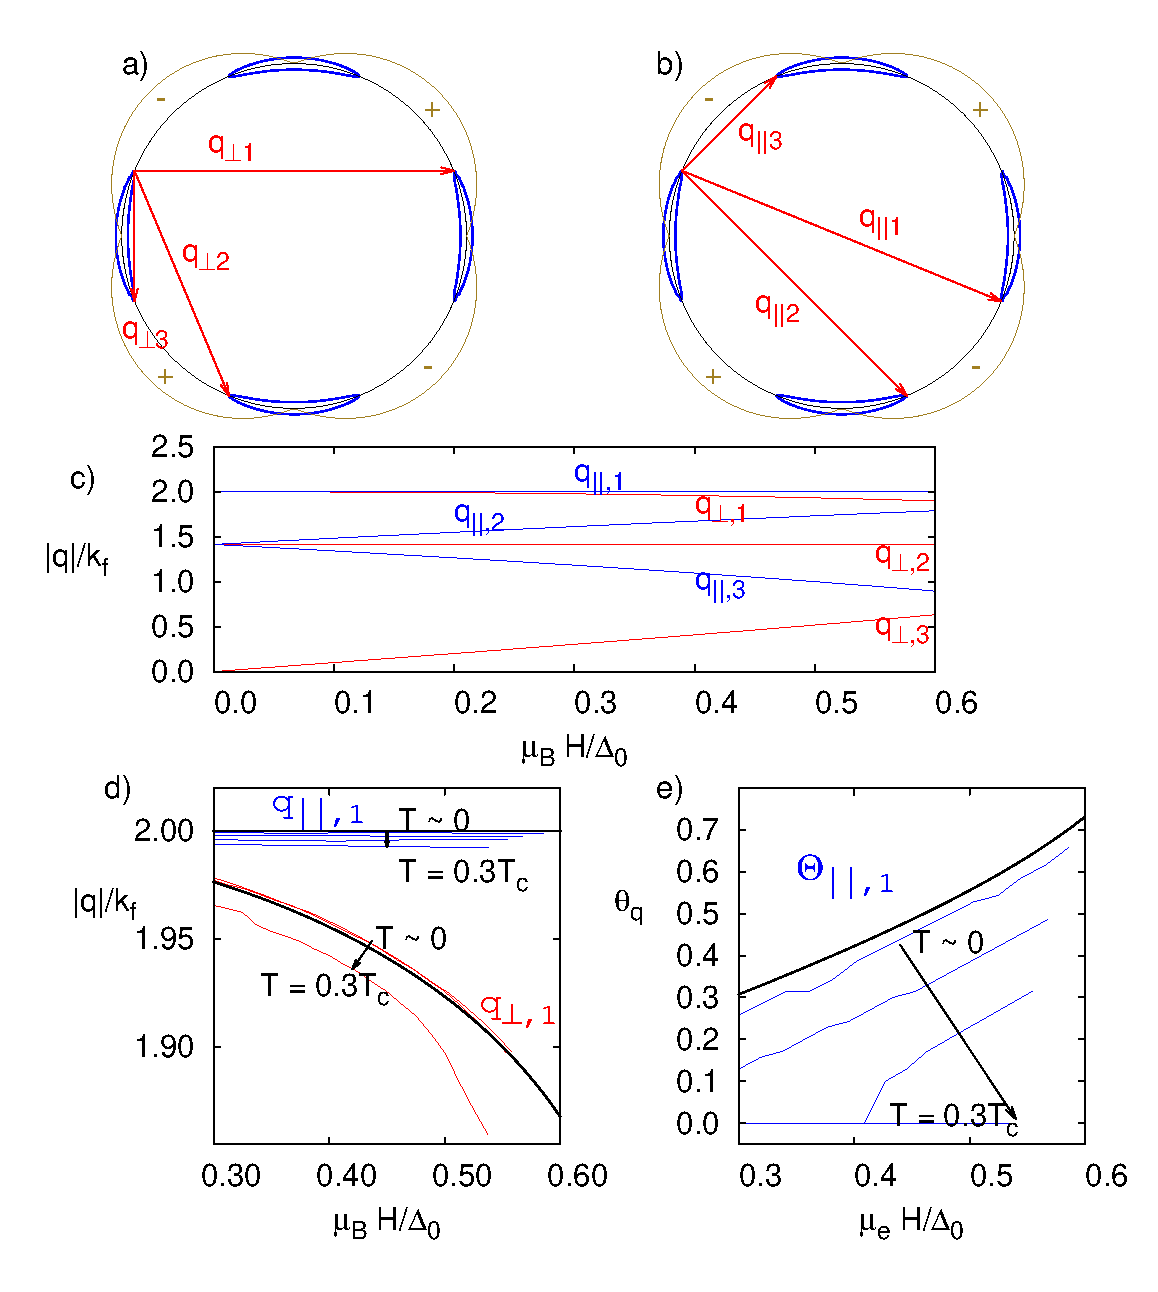
\includegraphics[width=0.95\linewidth]{Fig2.eps}
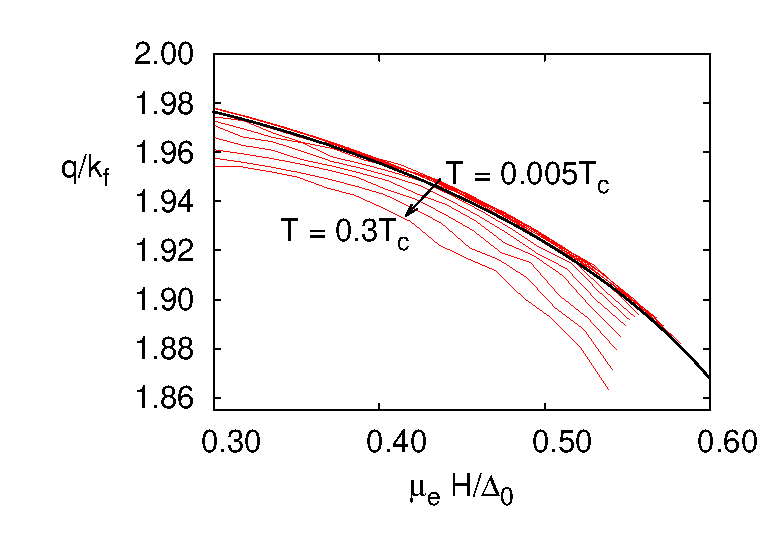
\includegraphics[width=0.75\linewidth]{Fig2d.eps}
\caption{ 
	\label{fig:qq} 
	\red{Ben, please unite these figures into 1 eps file, and label panels (a-d). For (d) use your figure with 
	both perpendicular and parallel wave vectors. Make (a,b) circles bigger, same size as square panels 
	(c,d) below them. Squeeze (c) and make sure to use same colors for q's in (c) and (d). } 
	(Color online) 
	Magnetic field produces pockets of low energy spin-down excitations near the nodes 
	of the order parameter (blue line regions). 
	The enhancement of the spin susceptibility in the d-wave superconductor occurs 
	when magnetization vector connects quasiparticle pockets with opposite sign gap 
	for transverse response (a), and same sign gap for longitudinal response (b). 
	(c) the magnitude of the magnetization vectors as a function of the field at zero 
	temperature, determined by geometry (a,b); 
	(d) finite temperature deviations of the optimal magnetization vector from (c). 
	\red{Ben: have you checked that the other wavevectors (beside $q_{\parallel 1}$ and $q_{\perp 1}$) 
	behave in the same way, i.e. with temperature they move such that the FS pockets overlap increases?} 
} 
\end{figure}
%%%%%%%%%%%%%%%%%%%%%%%%%%%%%%%%%%%%%%%%%%%%%%%%%%%%%%%%%%%%%%%%%%%%%%%%%%%%%%%%%

In the superconducting state we want to find the maximal values of susceptibility and the corresponding 
magnetization wave vectors. We concentrate on the superconducting state with $d$-wave symmetry. 
The presence of the nodes in the gap function - product of unconventional pairing, -  results in 
spin-down quasiparticles with negative energies. This gives new Fermi surface pockets near the nodes 
of $\Delta_\vk$, and partially destroys superconductivity (Pauli pair breaking). 
The $\vq \to 0$ limit gives the well-known diamagnetic response, which in unconventional superconductors 
is modified due to the nodal quasiparticles, $\chi(0)/\chi_0 \sim \mu_\sm{B} H_0/\Delta_0$.  

A look at different terms in Eqs.~(\ref{eq:chi}) provides a reasonable guess for 
wave vectors that 
might give the largest enhancement of the susceptibility. 
For longitudinal $\chi_\parallel$ it is the first term in the sum with $\mu=-1 (\downarrow)$, 
and for transverse $\chi_\perp$ this is the last term, also with $\mu=-1$. 
In these terms there is possibility of new spin-down Fermi pockets touching at a single point, 
and the Fermi functions in the numerator give non-zero contribution. 
To maximize the value of $\chi$ we can also use $\vq$'s that give the largest coherence 
factors. 
The most positive values of $ ( u_{\vk_+}u_{\vk_-}+v_{\vk_+}v_{\vk_-} ) $, 
and the largest contribution to longitudinal $\chi_\parallel$,  
are achieved when the magnetization vector $\vq$ connects 
hot spots lying in quadrants with the same sign of the gap $\Delta_{\vk_\pm}$, 
and thus the same sign of $v_{\vk_\pm}$. There are three such vectors. 
Similarly, largest $\chi_\perp$ is reached when $ ( u_{\vk_+}v_{\vk_-}-v_{\vk_+}u_{\vk_-} ) $
is most positive. This occurs at another three vectors, connecting hot spots with the 
opposite sign of $\Delta_{\vk_\pm}$. 
These vectors are shown in Fig.~\ref{fig:qq}(a),(b) for $\chi_\perp$ and $\chi_\parallel$. 
The $T=0$ length of the magnetization vectors as function of magnetic field 
is shown in Fig.~\ref{fig:qq}(c).

However, this guess has to be checked numerically, 
since the size of the new FS pockets is small, having energy scale of 
$\mu_\sm{B}H_0 \sim \Delta_0 \ll \epsilon_F$ 
and momentum space scale $1/\xi_0 \ll k_F$. This means that the changes with temperature 
and field to $\vq$s and to $\chi$ can be considerable, and difficult to treat 
analytically. 
As an example, in Fig.~\ref{fig:qq}(d) 
we show the $T$-induced deviations of optimal $\vq$ vectors from their $T=0$ values, 
found by numerically finding the maximum of the susceptibility $\chi(\vq)$, 
and corresponding $\vq$, at given $T$ and $H_0$. 
We note that at finite $T$ the magnetization vector is smaller than zero-$T$ one in 
both components, and results in bigger overlap of the Fermi pockets. 
\red{Ben, is this statement correct?}

 %%%%%%%%%%%%%%%%%%%%%%%%%%%%%%%%%%%%%%%%%%%%%%%%%%%%%%%%%%%%%%%%%%%%%%%%%%%%%%%%%
\begin{figure}[t]
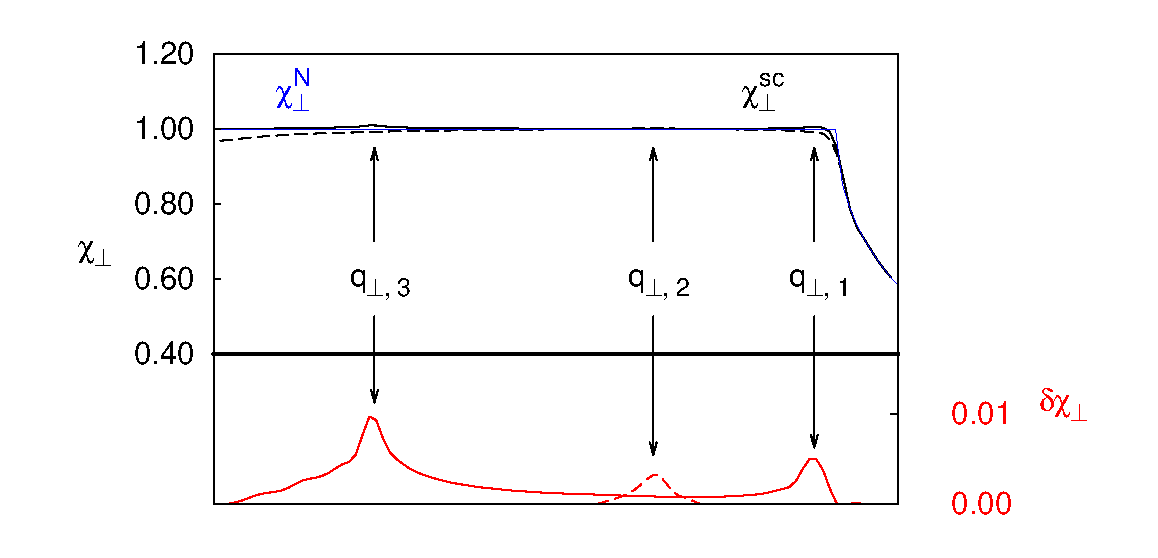
\includegraphics[width=0.95\linewidth]{Fig3.eps}
\caption{
	\label{fig:chi_enh}
	\red{Ben, insert some white space between perp and parallel panels and label them (a),(b).} 
	(Color online)
	(a) The $T=0$ normalized transverse susceptibility in the superconducting
state (red) as a function of $q$. For directions along $\vq_{\perp 1} || \vq_{\perp 3}$ (solid red) 
and along $\vq_{\perp 2}$ (dashed red), it shows enhancement over 
the normal state (blue) at values of the wavevectors 
$q_{\perp1}$, $q_{\perp 2}$ and $q_{\perp 3}$ shown in Fig.~\ref{fig:qq}(c). 
We use here  $\mu_\sm{B} H = 0.5\Delta_0$. 
The lower pane shows $\delta\chi_\perp(q) = \chi_\perp^{sc}(q) - \chi_\perp^{N}(q)$. 
The maximal enhancement occurs at wave vector $\vq_{\perp 3}$ and is of the 
order $\delta \chi_\perp/\chi_0 \sim \Delta_0/\epsilon_F = 0.1$ in this example. 
%
(b) Same for longitudinal component. 
Solid red for directions along $\vq_{\parallel 2} || \vq_{\parallel 3}$, and dashed for $\vq_{\parallel 1}$.  
Here we use $\Delta_0/\epsilon_F = 0.01$ 
as we found that this value corresponds to maximal increase of the $\chi(q)$ compared 
to the normal state value. 
\red{Ben: is this statement correct? Same $\mu_\sm{B} H = 0.5\Delta_0$ though?} 
}
 \end{figure}
%%%%%%%%%%%%%%%%%%%%%%%%%%%%%%%%%%%%%%%%%%%%%%%%%%%%%%%%%%%%%%%%%%%%%%%%%%%%%%%%%
  

In Fig.~\ref{fig:chi_enh} we plot the susceptibility as a function of magnetic wave vector 
in superconducting state at zero temperature and in 
magnetic field $\mu_\sm{B} H = 0.5\Delta_0$. 
The directions of the $\vq$s are chosen in accordance with Fig.~\ref{fig:qq}.  
The maximal enhancement of $\chi$ always correspond to the longest $\vq$. 
For the transverse component it is just below the normal state kink $k_{f\uparrow}+k_{f\downarrow}$, 
and maximal $\chi^{sc}_\perp(q)$ sits well above the maximal normal state value of $\chi_0$. 
For the longitudinal component the most enhanced peak is at nearly $2k_f$ - right between the two 
normal state kinks at $2k_{f\uparrow\downarrow} = 2k_f \sqrt{1\mp \mu_\sm{B}H_0/\epsilon_F}$, 
and as result although large, still does not go above the $\chi_0$ value of the 
normal state. 


%%%%%%%%%%%%%%%%%%%%%%%%%%%%%%%%%%%%%%%%%%%%%%%%%%%%%%%%%%%%%%%%%%%%%%%%%%%%%%%%%
\begin{figure}[t]
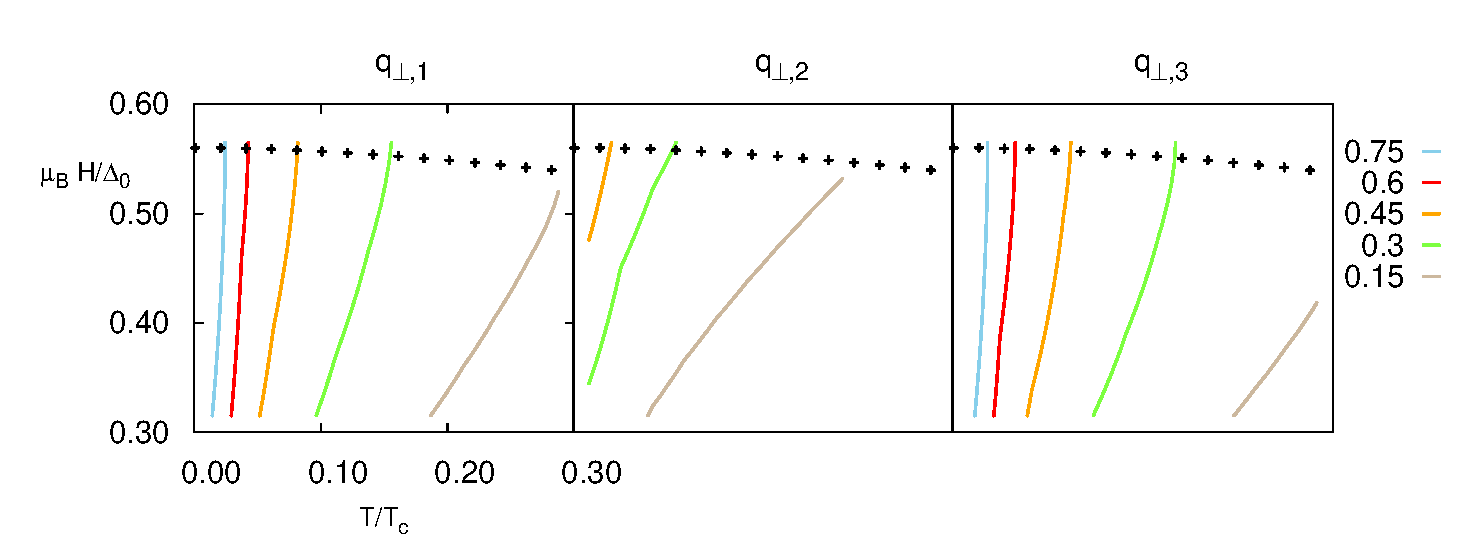
\includegraphics[width=0.95\linewidth]{Fig4.eps}
\caption{ 
	\label{fig:ph.d} 
	\red{Ben: I don't have the latest version of this figure. 
	Remove the upper row for $\Delta_0/\epsilon_F=0.1$. 
	Add as lower row phase diagrams for parallel $\chi$.
	Bigger fonts. 
	Are you sure that $q_1$ and $q_3$ give the almost the same phase diagram in terms of 
	contour locations? From Fig.~\ref{fig:chi_enh}(a) I see that the enhancement for 
	$q_3$ is 3 times smaller than that for $q_1$ - how can the countors be in the same place?
	Also remove the experimental line from the plots, and send me the data for that line. 
	Or even better: Insert Fig 1 into TH-phase diagram of Pauli limited d-wave 
	superconductor, and indicate the experimental Q-phase region, like you had for the 
	March meeting talk in xx\_maxsus\_diagram.eps. 
	} 
	(Color online) 
	Contour lines of maximal enhancement of susceptibility in the $T$-$H$ 
	phase diagram. Different contours correspond to relative enhancements 
	$\delta\chi(q)/\chi_0$ given in percents. 
	Upper row is for transverse $\chi_\perp$ for three wave vectors shown in figure \ref{fig:qq}(a). 
	Lower row is for longitudinal $\chi_\parallel$ for wave vectors in Fig.~\ref{fig:qq}(b). 
	The black bold dotted line is the first order phase transition
	for a Pauli limited $d$-wave superconductor, and the bold red line is a
	qualitative sketch of the Q-phase boundary of CeCoIn$_5$.  $\Delta_0 =
	0.005\epsilon_f$ 
}
\end{figure}
%%%%%%%%%%%%%%%%%%%%%%%%%%%%%%%%%%%%%%%%%%%%%%%%%%%%%%%%%%%%%%%%%%%%%%%%%%%%%%%%%
 
%~~~~~~~~~~~~~~~~~~~~~~~~~~~~~~~~~~~~~
%\emph{Conclusions.}
%~~~~~~~~~~~~~~~~~~~~~~~~~~~~~~~~~~~~~
%
Finally, we present $T$-$H$ phase diagram of a $d$-wave superconductor with Pauli pairbreaking, 
and plot the the contours of maximal susceptibility enhancement in Fig.~\ref{fig:ph.d}. 
We find the self-consistent value of the 
gap amplitude $\Delta_\vk = \Delta(T,H) \sin2\theta_\vk$, (Note $\Delta_0 = \Delta(0,0)$) 
at each $T$ and $H_0$, and then substitute it into Eq.~(\ref{eq:chi}). 
Then we scan over magnetization vectors close to suggested $\vq_i$ to find the maximal value of 
$\chi(\vq)$. In this way we find the optimal wave vector and corresponding maximal $\chi$ for 
given $T$,$H$. 
\red{Ben: is this is the correct description of procedure? or you find max value of $\delta \chi$ or 
something else? - please describe your procedure!}

The magnitude of the $\delta \chi$ becomes positive and increasing as we go to the 
upper left corner (low $T$, high $H$). The fact that susceptibility in the superconducting state 
is larger than the normal state maximum $\chi_0$ indicates that the superconducting state 
may naturally ``attract'' and host a magnetic phase while the normal state remains non-magnetic. 
The many-body effects lead to the expression for susceptibility in terms of the 
bare $\chi$ that we calculate, 
$\chi^{RPA}_{\alpha\beta}(\vq)={\chi_{\alpha\beta} (\vq) }/{[1-J(\vq) \chi_{\alpha\beta}(\vq)]}$
and if the normal state is close to the magnetic instability, $J \chi_0 \lesssim 1$, 
a small increase in susceptibility 
in the superconducting state $\delta\chi/\chi_0 \sim \Delta_0/\epsilon_F$ 
may induce the magnetic instability. The curves of constant 
$\delta\chi(T,H)$ will determine the boundary of the magnetic SDW 
state inside the superconducting phase. 

The slope and the direction of $\delta\chi$ increase in the $T$-$H$ phase diagram is consistent with 
the location of the Q-phase transition in \cecoin, and agrees with the conclusions of 
\cite{sc_afm_kato}. 

We also note the field dependence of the various critical $\vq$'s identified in
this paper (Fig.~\ref{fig:qq}(c,d)), which has not been addressed in many of
the other theories which try to explain the origins of the Q-phase of
CeCoIn$_5$. Experimental evidence points to a near constant or possibly
increasing $|\vq|$ which is consistent with $\vq_{\perp,2}$, $\vq_{\perp,3}$,
$\vq_{\parallel,1}$ or $\vq_{\parallel,2}$.
\cite{sc_sdw_anton,mag_afm_fflo_sigrist,fflo_pen_depth,sc_afm_kato,sc_afm_ikeda,sdw_vortex,
cecoin5_Kenzelmann2}

In conclusion, we investigated the behavior of spin susceptibility in Pauli-limited 
unconventional superconductors. We found that the field-induced nodal quasiparticles, and the sign-changing 
nature of the gap, leads to the enhancement of the transverse susceptibility component 
inside the superconducting phase. 
As a result, similar enhancement in conventional superconductors, even with strongly anisotropic and even nodal 
gap function, is unlikely. 
The enhancement is of the order $\delta\chi/\chi_0 \sim \Delta_0/\epsilon_F$ 
and is a strong function of temperature and magnetic field; 
it may result in SDW order formed inside the superconducting phase at low temperatures and 
high fields, consistent with observations in \cecoin.  
There are several magnetization vectors that connect field-induced Fermi pockets. 
Enhancement of the longitudinal component is also significant but it occures on the 
background of fast-decreasing normal state $\chi_\parallel^N(\vq)$ and does not lead to 
significant increase over $\chi_0$. 

This research was done with NSF support through grant DMR-0954342. 
 %~~~~~~~~~~~~~~~~~~~~~~~~~~~~~~~~~~~~~~~~~~~~~~~~~~~~~~~~~~~~~~~~~~~~~~~~~~~~~~~
  %~~~~~~~~~~~~~~~~~~~~~~~~~~~~~~~~~~~~~~~~~~~~~~~~~~~~~~~~~~~~~~~~~~~~~~~~~~~~~~~
   %~~~~~~~~~~~~~~~~~~~~~~~~~~~~~~~~~~~~~~~~~~~~~~~~~~~~~~~~~~~~~~~~~~~~~~~~~~~~~~~
    %~~~~~~~~~~~~~~~~~~~~~~~~~~~~~~~~~~~~~~~~~~~~~~~~~~~~~~~~~~~~~~~~~~~~~~~~~~~~~~~
     %~~~~~~~~~~~~~~~~~~~~~~~~~~~~~~~~~~~~~~~~~~~~~~~~~~~~~~~~~~~~~~~~~~~~~~~~~~~~~~~
      %~~~~~~~~~~~~~~~~~~~~~~~~~~~~~~~~~~~~~~~~~~~~~~~~~~~~~~~~~~~~~~~~~~~~~~~~~~~~~~~

\bibliography{mybib}

%~~~~~~~~~~~~~~~~~~~~~~~~~~~~~~~~~~~~~~~~~~~~~~~~~~~~~~~~~~~~~~~~~~~~~~~~~~~~~~~%
\end{document}
%~~~~~~~~~~~~~~~~~~~~~~~~~~~~~~~~~~~~~~~~~~~~~~~~~~~~~~~~~~~~~~~~~~~~~~~~~~~~~~~%
